\section{Background}

\begin{figure}[t]
\begin{center}
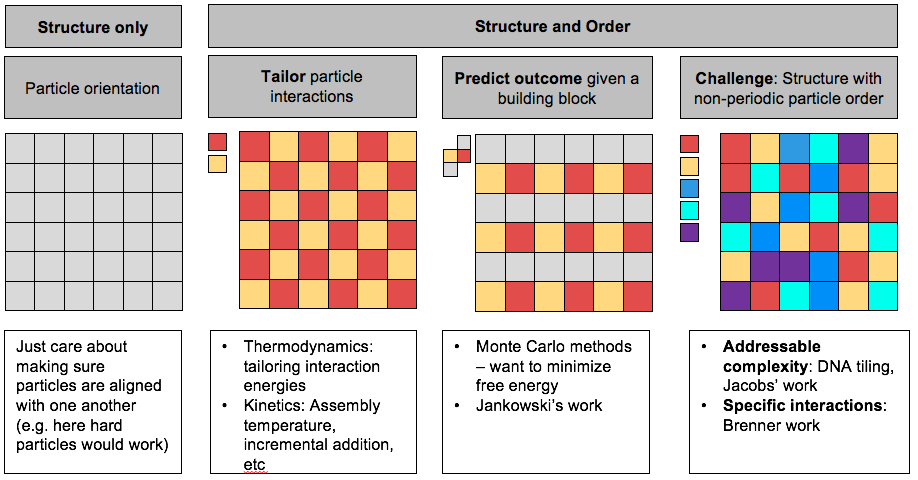
\includegraphics[width=6.5in]{../figures/litreview.png}
\caption{Demonstration of the state of the art in the literature}
\label{fig:litreview}
\end{center}
\end{figure}

Let's take a simple system and use it to illustrate the state of the art in the theory for engineering self-assembly behavior.

Let us say that we have the simple target 2D array shown in Figure \ref{fig:litreview}.

% =====
% STRUCTURE ONLY
% ====
\subsection{Directing structure}
If we assume all the particles in our system are uniform, we simply care about making sure particles assemble into the target structure.
As in any type of assembly, this implies a minimization of free energy.
In the example of hard squares above, minimization of free energy corresponds to a maximization of entropy.

\begin{itemize}
\item Archimedean tilings
\item Glotzer work on assembling target structures
\end{itemize}


\cite{vanAnders_2014_ACSNano}: Can treat shape as giving particles an effective entropic patchiness

\cite{Millan_2014_ACSNano}:
Develop a metric of self-assembly complexity, flow chart in Figure 3.
Archimedean tilings (ATs)
Here, we report the minimal set of interactions needed to self-assemble experimentally accessible ATs from regular polygons, mimicking nanoplates assembled into crystalline monolayers (Figure 1). We show through Monte Carlo simulations the self-assem- bly of these tilings by exploiting entropic and enthalpic interactions encoded in the shape of the polygons. We arrive at a design strategy for patchy polygon particles that is accessible to current experimental techniques and present the minimal set of design rules for each AT. We report that four ATs, namely, the (63), (36), (44), and (3.122) tilings, can be assembled solely with hard interactions, highlighting the role of directional entro- pic forces39,40 that arise from the particle shape.

After selecting the building blocks, the design pro- cess examined the constituent polygonal building blocks and alters the interaction complexity by chan- ging the specificity of interactions. The four models ranked in terms of specificity are hard, symmetric patches, shape-specific patches, and edge-specific patches

Manually adds complexity in the amount of specificity:
Initially, we test if entropic interactions are sufficient to self-assemble each crystalline structure. If the infinite pressure ground state (hard particle) won't assemble the target structure, add attractive interactions. If the crystalline structure for a mixture of building blocks does not contain the alternating building block property, it is necessary to use edge-specific interactions.


% =====
% STRUCTURE AND ORDER: TAILORING PARTICLE INTERACTIONS
% ====
\subsection{Directing structure and particle order}
As we look to make more complex materials, though, we also want to specifically order the particles within a structure.
We can approach this through tailoring the thermodynamics and/or the kinetics.

\begin{enumerate}
\item BUBBA work
\item DNA tilings / DNA origami
\item Protein origami
\item DNA-tailored assembly
\item need to find some other citations here?
\end{enumerate}

\begin{enumerate}
\item \cite{Jankowski_2009_JChemPhys,Jankowski_2011_JPhysChemB,Jankowski_2012_SoftMatter}
\item Design and self-assembly of two-dimensional DNA crystals \cite{Winfree_1998_Nature}, primer to DNA origami \cite{Castro_2011_Nature}, Programming Self-Assembly of DNA Origami Honeycomb Two-Dimensional Lattices and Plasmonic Metamaterials \cite{Wang_2016_JACS}, Designer nanoscale DNA assemblies programmed from the top down \cite{Veneziano_2016_Science}
\item Proteins can now also be designed, ala DNA origami: \cite{Huang_2016_Nature}
\item \cite{Mirkin_1996_Nature,Park_2008_Nature,OBrien_2016_JACS,Liu_2016_Nature}, DNA-guided crystallization of colloidal nanoparticles \cite{Nykypanchuk_2008_Nature}
\end{enumerate}


\cite{Park_2008_Nature}: can create crystals using DNA functionalization
\cite{OBrien_2016_JACS}: Colloidal crystallization can be pro- grammed using building blocks consisting of a nano- particle core and DNA bonds to form materials with controlled crystal symmetry, lattice parameters, stoichiometry, and dimensionality. Can tailor DNA length and shape to get different crystal structures

DNA programmable assembly. The sequence-specific binding property of DNA can be applied to direct the assembly behavior of colloidal particles at the nanoscale. This is a powerful strategy to control nanomaterial assembly because it allows tuning of the interparticle interaction in highly specific ways. For example, attaching DNA linkers with self-complementary sequences to particles directs them to maximize the number of nearest neighbors, resulting in fcc arrangement. On the other hand, particles with non-self-complementary linkers, which only allow A-B contacts, assemble into bcc or CsCl-type arrangement by maximizing the number of A-B contacts around the first coordination shell \cite{Park_2008_Nature}.This technique has recently been applied to anisotropic particles and opened possibilities to access diverse crystal structures in nanoscale by employing the DNA programmability as well as geometrical properties of the anisotropic shapes (25, 26).Despite its powerful potential, studies regarding the assemblies of DNA-coated anisotropic colloids have until recently (Sangmin's paper) been limited to simple crystal structures with small unit cells (27, 28). 

% =====
% STRUCTURE AND ORDER: PREDICTING ASSEMBLY
% ====
\subsection{Predicting assembly of complex building blocks}

Easy enough for hard particles, such as looked at in \cite{Damasceno_2012_Science}.
To test the interactions we've tailored above, we also need to be able to test the assembly properties of these building blocks.
We want to see what structure they will assemble into to minimize their free energy.
Our initial instinct would be to run these simulations to steady state or equilibrium.
However, systems with complex interactions such as these can get themselves caught in metastable free energy local minima that MC methods may not have large enough energy fluctuations to escape from.
This is where thermodynamics and kinetics really come to play together

\begin{itemize}
\item BUBBA work
\item Wales work (disconnectivity graphs) - more of the thermo
\item Kinetic pathway design - Frenkel, Jacobs
\item Connectivity graphs to show the order of assembly
\item Pathway assembly sampling
\item swear I read something earlier today about metastable/kinetic traps
\end{itemize}



% =====
% STRUCTURE AND ORDER: THE BIG CHALLENGE
% ====
\subsection{Challenge: Self-assembly of complex structures}

Real-world:
\begin{itemize}
\item Protein assembly
\item Complex DNA tiling, assembly - Mirken, Winfree, Rutherford, check semisynbio sources
\end{itemize}

\textbf{Motivation 1: DNA assembly, DNA tiles, DNA cubes}

Taken from intro of \cite{Reinhardt_2014_PRL}: \\
The observation by Ke et al. [Science 338, 1177 (2012)] that large numbers of short, predesigned DNA strands can assemble into three-dimensional target structures came as a great surprise, as no colloidal self-assembling system has ever achieved the same degree of complexity.
That failure seemed easy to rationalize: the larger the number of distinct building blocks, the higher the expected error rate for self-assembly.
The experiments of Ke et al. have disproved this argument.
Here, we report Monte Carlo simulations of the self-assembly of a DNA brick cube, comprising approximately 1000 types of DNA strand, using a simple model.
We model the DNA strands as lattice tetrahedra with attractive patches, the interaction strengths of which are computed using a standard thermodynamic model.
We find that, within a narrow temperature window, the target structure assembles with high probability.
Our simulations suggest that misassembly is disfavored because of a slow nucleation step.
As our model incorporates no aspect of DNA other than its binding properties, these simulations suggest that, with proper design of the building blocks, other systems, such as colloids, may also assemble into truly complex structures.


\textbf{Motivation 2: Protein folding}

\subsection{Theory perspective}:
\begin{itemize}
\item Addressable complexity
\item Efficiency of specific interactions
\end{itemize}

From \cite{Wales_2017_JChemPhys}:
To construct an operational machine, we generally need to assemble a variety of components into a well-defined spatial arrangement. The experimental realisation1 of programmed self-assembly for a structure composed of thousands of dis- tinct building blocks has therefore generated great interest. Here the building blocks are ?DNA bricks,? which can bind by hybridisation to four neighbours. The resulting assemblies are considered ?addressable,? in that the different components are located in specific local environments. Understanding and developing design principles for such structures could pro- vide a route to translation of information encoded in nanoscale building blocks into new materials with a specific structure and function. Developing models that reproduce the key exper- imental results using the simplest possible representations is therefore an important challenge, and initial efforts for DNA bricks have already reproduced addressable assembly for as many as 1000 distinct components.2 Recent insight into computer simulation indicates that robust self-assembly may require precise conditions for nucleation to occur. The yield for the target structure can be improved significantly using a specific annealing protocol.3

\textbf{Information as a measure of the likelihood of a particular configuration being preferred.}
In 2015, a review article in \textit{Nature Physics} (which has since been cited 255 times) reviewed the state of the art on applying information theoretic entropy-- i.e. Shannon entropy-- as a way of understanding non-equilibrium thermodynamics \cite{Parrondo_2015_NaturePhysics}.
In this work, they investigate information entropy as a placeholder for non-equilibrium entropy production.
This entropy production gives an overall likelihood of a configuration (one which minimizes the non-equilibrium free energy of a system while maximizing the non-equilibrium entropy).
However, this method applies to the overall structure, or the overall likelihood of a structure being the preferred structure.

Some authors have gone so far as to suggest replacing the thermodynamic concept of entorpy with information \cite{AFarewelltoEntropy}.

\textbf{``Addressable complexity'' seeks to engineer pathways for particular particles to reach their destination.}
Low free energies of a target structure, however, do not guarantee efficient assembly.
There are a number of ways addressing this problem in the literature.
One way of forcing systems into assembly is to design a free energy landscape that minimizes such meta-stable traps \cite{Wales_2017_JChemPhys}.
Competition between degenerate structures of equivalent potential energy was reported for clusters of six attractive spherical colloids, where symmetry breaking leads to higher rotational entropy of the less symmetric conformation, resulting in lower free energy \cite{Meng_2010_Science}.

Taken from \cite{Jacobs_2015_JChemPhys}: 
A well-known example of addressable complexity-- that is, specific binding-- can be found in ``one-pot'' DNA self-assembly of DNA tiles, which use the hybridization of complementary DNA sequences to construct complex structures consisting of hundreds of subunits from a single soup of monomers \cite{Ke_2012_Science}.
Simulation results have shown that such one-pot self-assembly can succeed with highly simplified model subunits that lack the molecular details of DNA tiles, suggesting that similar design strategies should be widely applicable \cite{Reinhardt_2014_PRL}.
In the work by Jacobs \textit{et al}, they had particles with designed interactions between one another.
They represented the target bonds by a graph, $G$.
However, this model is based on the assumption that ``designed interactions in the target structure are typically much stronger than any incidental associations between sub-units that should not be connected in the final assembly''.
This is a fine assumption for their proof of concept, but is not valid in real-world system.
As a concrete example, protein-folding is perhaps the most well-explored biological system that assembles due to specific interactions \cite{Dill_1993_CurrOpinStructBiol}.
However, one of the major challenges to solving the protein-folding problem are competing ``cross-talk'' interactions [CITATIONS NEEDED; chaperoned folding and assembly Chakrabarty 2017].

In later work, Jacobs et al addressed this oversight and accounted for incidental interactions in addition to designed interactions \cite{Jacobs_2015_PNAS}.


Low energies may not guarantee efficient assembly
compartmentalized, multi-stage assembly
grannemana and baserga 2004

Talk outline:
1. self-assembly kinetics can be rationally designed-- leverage thermodynamics
2. evolution has already selected for optimal assembly pathways in complex biomolecules


\textbf{Specific binding interactions can be tailored to lead to target structures}.
However, there is a delicate balance of specificity required.
On the over-specified side, we have bonds that are specific to their intended neighbor with probability 1.0.
On the under-specified side, we have non-specific interaction patches that will bond to any other patch with probability $1/n$, where $n$ is the total number of patches in the system.

In work from our group, Eric Jankowski sought to generate energy-minimizing configurations for such patchy particles \cite{Jankowski_2009_JChemPhys} in a process he called ``bottom-up building block analysis'', or BUBBA.
Cluster Monto Carlo (cMC) and LAcMC methods are relatively poor methods for finding potential energy minima formed from patchy particles with disparate interaction energies due to their tendency to become trapped in metastable configurations as well as the low degeneracy of potential energy-minimizing configurations (Q).
BUBBA effectively searches a subset of the configuration space for energy-minimizing configurations.
Jankowski predicted that that BUBBA would be useful for evaluating many different particles for self-assembly ``propensity''.

Partition functions encode all the thermodynamics of a system, but for most systems of practical importance they cannot cannot be calculated exactly.
This is due to many indistinguishable degenerate states. 
In the cases where small numbers of distinguishable configurations comprise a majority of a partition functions' weight, as is the case for systems at low temperatures and for many anisotropic building blocks with disparate interactions, BUBBA is a particulalry effective method for generating partition functions that have been heretofore inaccessible. 
This allows us to ask ``What structures are thermodynamically favored for this building block at any temperature?'' to be answered independently of assembly kinetics. \cite{Jankowski_2011_JPhysChemB}

% Note: Jankowski_2011_JPhysChem has a really good introduction

Both thermodynamic and kinetic barriers to assembling target structures.

Let's first look at a paper from the Brenner group, the ``Information capacity of specific interactions' \cite{Huntley_2016_PNAS}.
Their main thesis is that specific binding interactions have energetics that allow binding to occur with measurable probability.
Thus, we can measure the relative information in different types of binding.
This is more in line with the communication theory view of information (rare events giving more information) than it is with the materials view of information, in which high information events imply high probability of a desired event happening.

Our group, and many others in the materials community, are looking to engineering materials to control their structures, behaviors, etc.
A common method of engineering these materials is by tailoring the interactions between their components through chemistry, shape, etc.
By understanding how much \textit{assembly information} can be contained in these interactions, we can:
\begin{enumerate}
\item Compare the efficacy of different types of interactions in delivering desired behavior(s)
\item Theoretically predict the efficacy of new types of interactions
\end{enumerate}

Let's take the example of a lock and key system.
\textcolor{red}{ADD SECTION ON BRENNER PAPER FROM LIT REVIEW LAST YEAR}

However, we can use the concept of \textit{mutual information} in defining how much information is stored in an interaction in an intuitive manner.
(See notes on the Brenner paper below.)
Mutual information $I(X;Y)$ is a global measure of interaction specificity in systems with many distinct species.
It quantifies how predictive the identity of a lock $x_i$ is to the identity of key $y_i$ found bound to it.

